\chapter{Introduction to Markov Chain Monte Carlo and Bayesian Inference}

In this chapter, the basic theory of Markov chain Monte Carlo algorithms will be introduced, with an example provided alongside visualizations. Afterwards, the idea of Bayesian inference will be explained, including the instantiation of this problem using the Markov chain Monte Carlo algorithm.

\section{The Idea of Markov Chain Monte Carlo}
Markov chain Monte Carlo (abbr. MCMC) is an algorithm that performs sampling. General usage of the Markov chain Monte Carlo algorithm started in the fields of chemistry, biochemistry, and physics up until after 1990 when it was also adopted by the field of statistics and scientific computing~\cite{mcmc_handbook}. The general idea of the Markov chain Monte Carlo includes, as its name suggests, a combination of the Monte Carlo methods and the usage of Markov chains. The Monte Carlo methods solve numerical problems by repeatedly generating random numbers~\cite{monte_carlo_methods}, whereas the Markov chains provide this algorithm a property so that each sample that is generated depends on the sample that is generated before~\cite{mcmc_wang}.

The Markov chain Monte Carlo tries to sample an unknown target distribution using a proposal distribution that completely lies above the target distribution. The selection proposal distribution is crucial to the success of the algorithm, since it may lead to different behaviors of convergence and acceptance rate~\cite{mcmc_handbook}. The core of the Markov chain Monte Carlo is the application of a Markov chain, where the Monte Carlo integration is used. Given a distribution $\pi(\cdot)$ and its probability function $f(\cdot)$, a typical Monte Carlo simulation would perform the following mathematical approximation:
\begin{align}
\mathbb{E}[f(X)] \approx \frac{1}{n}\sum_{i=1}^{n}f(X_i)
\end{align}
where $\{X_i | i\in[1, n]\}$ is the sample space that is drawn from the distribution $\pi(\cdot)$~\cite{mcmc_practice}. Since this approximation is used on a Markov chain, each sample from the sample space is dependent on the sample before. In Markov chain Monte Carlo, this dependence is given by a transition kernel that is essentially a conditional distribution $\Pr[X_{i+1}|X_i]$~\cite{mcmc_practice}. In other words: After the last sample was generated, a distribution that takes this generated sample as a parameter is created. The next sample is then generated based on this newly created sample, which creates a dependence between both samples. Markov chains Monte Carlo functions thanks to a property called ergodicity that is shared by all Markov chains. The ergodic theorem states that the distribution of the states on the chain converges to a certain stationary distribution regardless of the starting state, as time approaches infinity~\cite{ergodicity}. This property could be applied in the case of Markov chain Monte Carlo as well. The starting states that do not sample from the stationary distribution before the ergodic states can be regarded as "burn-in states" and should be discarded. Thus, the approximation of the Monte Carlo simulation can be altered to
\begin{align}
\mathbb{E}[f(X)] \approx \frac{1}{n-b}\sum_{i=b + 1}^{n}f(X_i)
\end{align}
where $b$ denotes the position of the last state in the burn-in phase that should be discarded~\cite{mcmc_practice}. The determination of the burn in phase plays an important part in terms of the sample space accuracy and will be discussed later in this thesis in a more detailed manner.

A crucial prerequisite of the Markov chain Monte Carlo algorithm is the detailed balance condition. The ergodicity property after the burn-in period for every Markov chain can be mathematically defined as:
\begin{align}
\forall X, Y\in S. \ \pi(X) \Pr[Y|X] = \pi(Y) \Pr[X|Y]
\end{align}
\cite{mcmc_practice} where $S$ is the set of the state of a Markov chain. From this equation, we can derive the following property:
\begin{align}
\int \pi(X) \Pr[Y|X] dX= \int \pi(Y) \Pr[X|Y] dX =\pi(X_j)
\end{align}
What this equation essentially points out is that if $X$ is sampled from the stationary distribution $\pi(\cdot)$, $Y$ will also be from this stationary distribution~\cite{mcmc_practice}. This corresponds to the idea of ergodicity and proves that using the detailed balance equation, all of the subsequent samples will eventually connect stationary and target distribution from the very beginning.

\section{The Metropolis-Hastings Algorithm}
Metropolis-Hastings is a widely used algorithm that performs Markov chain Monte Carlo sampling. It is extremely versatile and often used to sample multivariate distribution. It was extensively used in the physics field, but later on also in the statistics field~\cite{understanding_mh}.

As mentioned before, the Markov chain Monte Carlo algorithms use a transition kernel to create dependence between two states.

The main idea is that for each iteration, a sample is drawn from the target distribution. For the generation of the next state, a distribution that takes the last sampled data point as a parameter will be created so that the new sample can be drawn from the newly created distribution~\cite{mcmc_practice}. An acceptance probability is then calculated using the following formula:

\begin{align}
\alpha(X, Y) = \min (\frac{\pi(Y)q[Y|X]}{\pi(X)q[X|Y]}, 1)
\end{align}
where $q[X|Y]$ denotes the proposal density from $X$ to $Y$. With the proposal density multiplied by the acceptance probability, the transition probability is derived:

\begin{align}
\Pr[X|Y] = q(X|Y) A(Y, X)
\end{align}
Due to the detailed balance equation~\cite{mcmc_practice}:
\begin{align}
\pi(X) q(Y|X) A(X, Y) = \pi(Y) q(X|Y) A(Y, X)
\end{align}
Bringing the ratio of the acceptance probability to the left
\begin{align}
\frac{A(Y, X)}{A(X, Y)} = \frac{\pi(Y)q[Y|X]}{\pi(X)q[X|Y]} := \alpha(X, Y)
\end{align} 
As we can see, the acceptance probability of the Metropolis-Hastings algorithm is calculated based on the ratio of the acceptance density from the old to the newly generated sample point to the acceptance density from the newly to the old generated sample point. However, since the probability space adds up to one, the maximum acceptance probability can not exceed one. Therefore, a minimum condition must be added.

A special case of the Metropolis-Hastings algorithm is the Metropolis algorithm. The Metropolis algorithm applies a symmetric distribution as the transition kernel, such as a normal distribution~\cite{metropolis}. Due to the symmetry, the proposal density $q[Y|X]$ equals to $q[X|Y]$. The idea is that the position of the density of the newly generated sample in the normal distribution centering the last generated sample is at the same altitude as the density of the last generated sample in the normal distribution centering the newly generated sample, as the visualization in Figure 2.1 suggests. 
\begin{figure}[H]
    \centering
    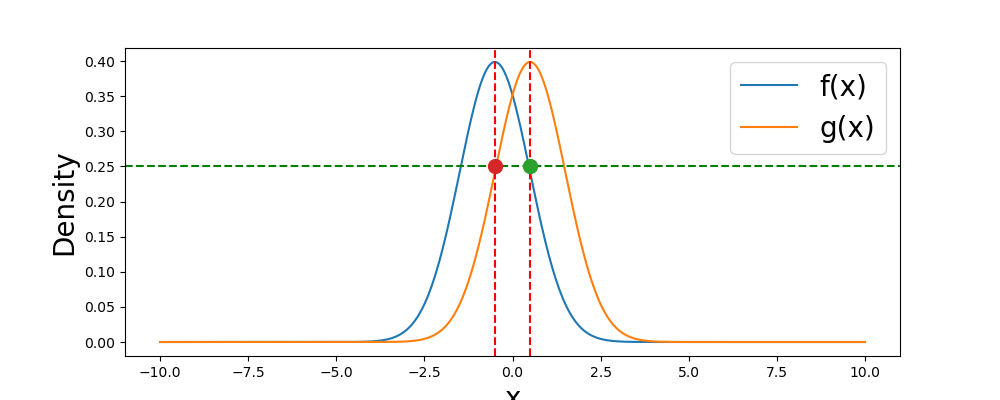
\includegraphics[width=0.8\textwidth]{figures/mcmc_example/proof.png}
    \captionsetup{width=.8\textwidth}
    \caption{Metropolis-Hastings algorithm with symmetric distribution as transition kernel}
    \label{fig:enter-label}
\end{figure}

In this graph, we can see that the green point is the newly sampled point conditioned on the distribution drawn by the last generated point. The red point denotes, on the contrary, the last generated point conditioned on the distribution drawn by the newly generated sample. These two points lie on the same level and share the equivalent value. Thus, the term $\frac{q[Y|X]}{q[X|Y]}$ cancels out to $1$. In this case, the acceptance probability becomes
\begin{align}
\alpha(X, Y) = \min (\frac{\pi(Y)}{\pi(X)}, 1)
\end{align}
which is virtually the ratio of the probability density of the newly generated sample to the probability density of the last generated sample. An illustration of this equation would be as follows: if $\pi(Y) > \pi(X)$, which means that the probability density of the newly generated sample is greater than its of the last generated sample, $\frac{\pi(Y)}{\pi(X)}$ is greater than $1$ and the acceptance of the newly generated point is guaranteed. Over time, the samples that are generated will have greater and greater probability density, and eventually, the peak will be reached. If $\pi(X) > \pi(Y)$, which means that the probability density of the newly generated sample is less than it's of the last generated sample, $\frac{\pi(Y)}{\pi(X)}$ is greater than $1$ and it is still probable to accept the newly generated point, however a less probability that is calculated equation~\cite{understanding_mh}.

\section{An example of the Metropolis-Hastings Algorithm}
In this section, an example of the Metropolis-Hastings algorithm will be given and visualized to provide an illustrative comprehension of the different steps of the algorithm. In this example, we want to sample an Erlang distribution from a normal distribution. We are set to generate 100,000 samples to compare how the generated samples fit the Erlang distribution. The Erlang distribution $f(x)$ has a shape of 3 and a scale of 2, whereas the normal distribution $g(x)$ has a mean of 10 and a standard deviation of 1.

\begin{figure}[H]
    \centering
    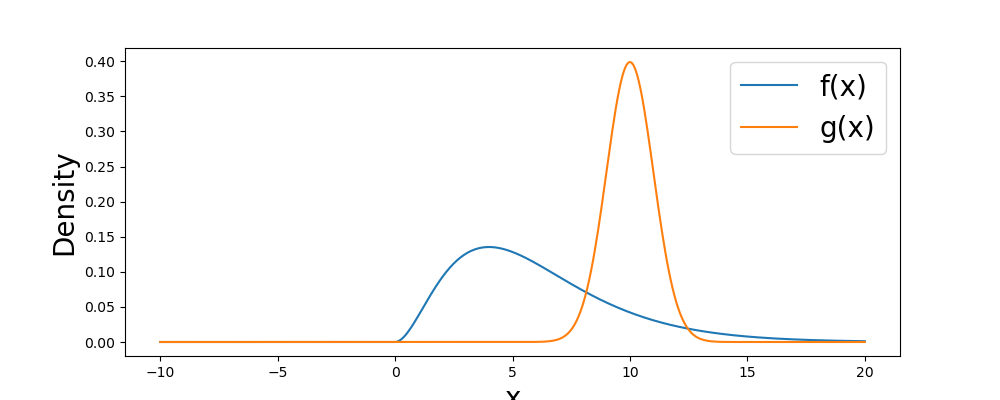
\includegraphics[width=0.8\textwidth]{figures/mcmc_example/first_step.png}
    \captionsetup{width=.8\textwidth}
    \caption{Scaling of the proposal distribution in the Metropolis-Hastings algorithm}
    \label{fig:enter-label}
\end{figure}


As we can see from Figure 2.2, the normal distribution that is sampled does not lie above the Erlang distribution. Therefore, we need to scale up the normal distribution. The scaled up graph is then shown in the Figure 2.3.

\begin{figure}[H]
    \centering
    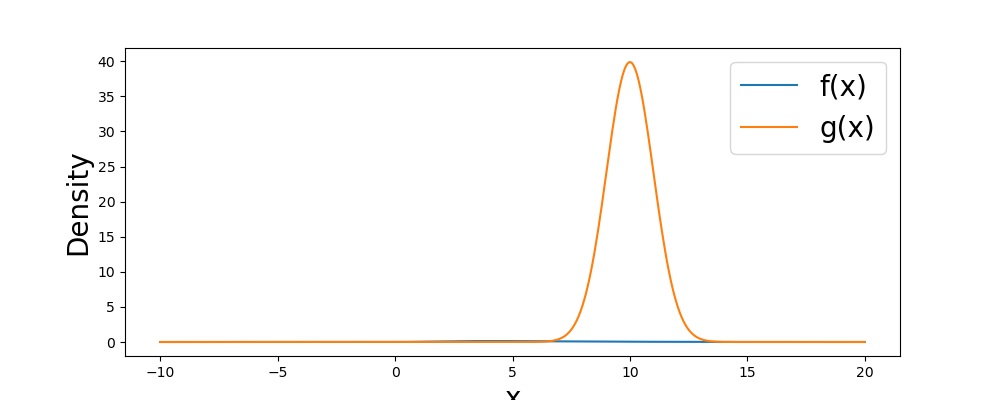
\includegraphics[width=0.8\textwidth]{figures/mcmc_example/second_step.png}
    \captionsetup{width=.8\textwidth}
    \caption{Scaling of the proposal distribution}
    \label{fig:enter-label}
\end{figure}



The transition kernel is set to be a normal distribution that sets the mean as the last generated sample and the standard deviation of 4. Since the normal distribution is symmetric, the acceptance probability could be set to $\alpha(X, Y) = \min (\frac{\pi(Y)}{\pi(X)}, 1)$, as mentioned above. The probability density function of the sampling distribution, $\pi(\cdot)$, is defined as follows:
\begin{align}
\pi(x) = \frac{1}{\sqrt{2\pi} \cdot \sigma}\exp(-\frac{(x-\mu)^2}{2\sigma^2})
\end{align}

where $\mu$ denotes the mean and $\sigma$ denotes the standard deviation of the normal distribution~\cite{densityFunction}.

We select 0 as our starting point and start the iterations from there on. In the first iteration, we acquire the random sample with the value of 1.5437347713886516. The acceptance probability is then $\alpha(X, Y) = \min (\frac{\pi(Y)}{\pi(X)}, 1) = 1$. In this case, since the acceptance probability is 1, it is guaranteed that this sample is accepted. We append this sample to the sample array and move on to the next iteration.

In the next iteration, we sample the value -1.802047900190033. The acceptance probability is then $\alpha(X, Y) = \min (\frac{\pi(Y)}{\pi(X)}, 1) = 0$. This means that this generated sample should by no means be sampled and we should carry on with the last sample. In this case, we repeat our old sample append it to the sample array, and continue.

We continue the rest of the iterations and draw a set of samples. If we plot the samples out and compare them with the target Erlang distribution, it would look something that the graph shown in Figure 2.4. As we can see, the samples that we generate resemble the targeted Erlang distribution. We can conclude that Markov chain Monte Carlo works perfectly in this specific example.

\begin{figure}[H]
    \centering
    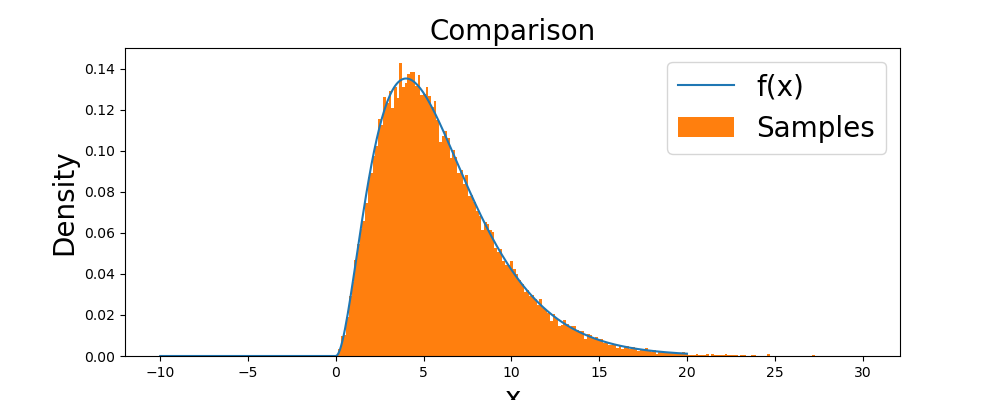
\includegraphics[width=0.8\textwidth]{figures/mcmc_example/result.png}
    \captionsetup{width=.8\textwidth}
    \caption{Posterior distribution derived from the Erlang distribution as proposal distribution}
    \label{fig:enter-label}
\end{figure}

\section{Advantages of Markov Chain Monte Carlo Methods over Other Commonly-Used Sampling Methods}
Markov chain Monte Carlo methods differ from other popular sampling methods and have specific advantages over them. In this section, the rejection sampling and the importance sampling are discussed and are compared to Markov chain Monte Carlo sampling.

Rejection sampling, also known as acceptance-rejection sampling, is a sampling method that generates samples that are independent from one another. Instead of generating the next sample from a newly created distribution that takes the last generated sample as input, the samples are generated from a sampling distribution that lies above the target distribution. The acceptance probability is than the ratio of the density of the target distribution over the sampling distribution~\cite{mcmc_practice}. However, if the target distribution is complicated, especially in multivariate cases, the ratio might be very low, causing the acceptance probability to be low as well, which leads to inefficiency. By creating a dependency between samples, Markov chain Monte Carlo methods avoid this inefficiency~\cite{ComparisonSampling}.

Importance sampling is a sampling method that is based on the calculation of weights. A typical implementation includes the generation of samples, calculating the weights of all of these samples, and calculating the expected value by summing them up together by the weights~\cite{ImportanceSampling}. The process of importance sampling is rather easy to implement. However, a disadvantage is that the samples that have higher weights dominate the calculation of the expected value, which essentially reduces the sample space since the samples that have lower weights play almost no role in the calculation. Markov chain Monte Carlo methods, on the other hand, eventually samples from the stationary distribution after the burn-in period, resulting in consistency of the sampling~\cite{ComparisonSampling}.

\section{The Idea of Parallel Implementation of Markov Chain Monte Carlo}
The objective of this thesis is to implement parallel versions of Markov chain Monte Carlo algorithms for the Bayesian inverse problem. Therefore, paralleling Markov chain Monte Carlo is a significant part of the thesis. The base idea is that instead of one single chain, several chains are run simultaneously~\cite{base_parallel}. Since after the burn-in period, every single state from each chain samples from the stationary distribution due to the ergodic property of the Markov chains~\cite{ergodicity}, all of the samples from different chains could be merged to present the target stationary distribution. However, other variations involve generating multiple points at the same time conditioned on the last generated sample and then evaluating the forward model~\cite{gpmh_broshure}. Since this chapter only provides an overview of the Markov chain Monte Carlo algorithm, a following chapter that is specifically dedicated to the parallel of the algorithm will be given.

\section{Introduction to Bayesian Inference}
The Bayesian inference problem is a method of statistical inference that is used to calculate the probability estimate based on evidence and the likelihood of the set of parameters~\cite{bayesian_inference}. Given a prior distribution that provides information on the preexisting data, the Bayesian inference problem uses the Bayes theorem to update the prior distribution using a likelihood function and derives the actual possibility.

Given the Bayes theorem~\cite{SatzBayes}:
\begin{align}
    \Pr[B|A] = \frac{\Pr[B]\cdot\Pr[A|B]}{\Pr[A]}
\end{align}
where $A$ and $B$ are two different incidents. This equation can than be formed into
\begin{align}
    \Pr[B|A] = \frac{\Pr[B]\cdot\Pr[A|B]}{\int\Pr[B]\cdot\Pr[A|B]dB}
\end{align}
$\Pr[A|B]$ is called the likelihood function, which is generated by a set of data to interpret how likely a particular set of observations is~\cite{likelihood_idea}. The $\Pr[B]$ is called prior, since this is the preexisting knowledge that is given~\cite{prior}. The denominator of the equation is called evidence, which is a constant that depicts the probability of observing the data across all values of the model parameters~\cite{mcmc_practice}. The result of the above equation is the posterior, which is the object of the Bayesian inference problem~\cite{mcmc_practice}.

The different implementations of the Bayesian inference problem are versatile and vary from one another. In this paper, we implement the Bayesian inference problem using the Metropolis-Hastings algorithm with a normal distribution transition kernel. The idea is that we calculate the acceptance rate based on the posterior calculation. For revision, the acceptance rate of the Metropolis-Hastings algorithm with a normal distribution transition kernel is given by~\cite{mcmc_practice}:
\begin{align}
    \alpha(X, Y) = \min (\frac{\pi(Y)}{\pi(X)}, 1)
\end{align}
Replacing $\pi(\cdot)$ with the posterior distribution, we derive:
\begin{align}
    \alpha(X, Y) = \min (\frac{\Pr[Y]\Pr[X|Y]}{\Pr[X]\Pr[Y|X]}, 1)
\end{align}
In plain language: The acceptance probability is calculated by the ratio of the prior and likelihood of the newly proposed point over the prior and likelihood of the last generated point. Since the evidence is a constant, they cancel each other out and will therefore not be taken into account.

Different variants of implementations are used throughout this paper to perform Bayesian inference of the hydrological model. They will be discussed in later chapters. For now, we will take a look at the hydrological model.





